\documentclass[convert={density=300,outext=.png}]{standalone}
\usepackage{tikz}
\usetikzlibrary{positioning}
\begin{document}
  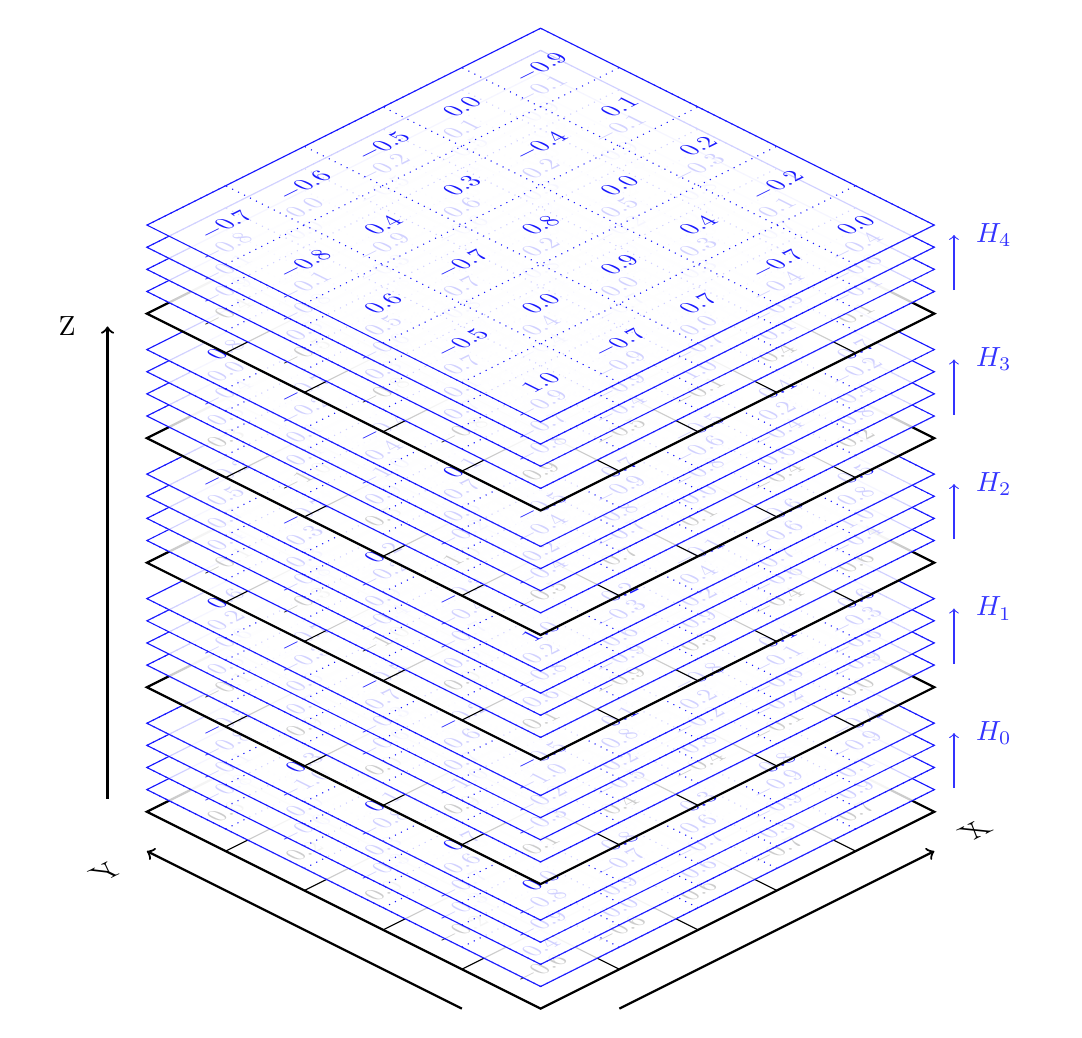
\begin{tikzpicture}[scale=1,every node/.style={minimum size=1cm},on grid]
    \def\heights{{-90,-45,0,45,90}}
	  \foreach \i in {0,...,4} {
      \pgfmathsetmacro{\x}{\heights[\i]}
      \begin{scope}[
        yshift=\x,every node/.append style={
        yslant=0.5,xslant=-1},yslant=0.5,xslant=-1
          ]
        %marking border
        \fill[white,fill opacity=0.8] (0,0) rectangle (5,5);
        \draw[step=10mm, black] (0,0) grid (5,5); %defining grids
        \draw[black, thick] (0,0) rectangle (5,5);%marking borders
        \pgfkeys{/pgf/number format/.cd, fixed, zerofill, precision = 1}

        \foreach \x in {0,...,4} {
          \foreach \y in {0,...,4} {
            \pgfmathsetmacro\rval{rand}
            \pgfmathparse{0.5+\x}
            \pgfmathresult \let\xpoint\pgfmathresult;
            \pgfmathparse{0.5+\y}
            \pgfmathresult \let\ypoint\pgfmathresult;
            \node[scale=0.8,thick] at (\xpoint,\ypoint)
              {$\pgfmathprintnumber{\rval}$};
          }
        }
      \end{scope} %end of drawing grids

      \foreach \z in {8,16,24,32} {
        \pgfmathparse{\z+\x}
        \pgfmathresult \let\zpt\pgfmathresult;

        \begin{scope}[
          yshift=\zpt,every node/.append style={
          yslant=0.5,xslant=-1},yslant=0.5,xslant=-1
            ]

          %marking border
          \fill[white,fill opacity=0.8] (0,0) rectangle (5,5);
          \draw[step=10mm, blue!90, dotted] (0,0) grid (5,5); %defining grids
          \draw[blue!90] (0,0) rectangle (5,5);%marking borders
          \pgfkeys{/pgf/number format/.cd, fixed, zerofill, precision = 1}

          \foreach \x in {0,...,4} {
            \foreach \y in {0,...,4} {
              \pgfmathsetmacro\rval{rand}
              \pgfmathparse{0.5+\x}
              \pgfmathresult \let\xpoint\pgfmathresult;
              \pgfmathparse{0.5+\y}
              \pgfmathresult \let\ypoint\pgfmathresult;
              \node[scale=0.8,thin,blue!90] at (\xpoint,\ypoint)
                {$\pgfmathprintnumber{\rval}$};
            }
          }
        \end{scope} %end of drawing grids

      }

      \begin{scope}[yshift=\x]
        \draw[blue!80,->] (5.25, 2.8) -- (5.25, 3.5) node[anchor=west] {$H_{\i}$};
      \end{scope}
    }

    \begin{scope}[
      yshift=-90,every node/.append style={
      yslant=0.5,xslant=-1},yslant=0.5,xslant=-1
        ]
      \draw[thick,->] (0.5,-0.5) -- (4.5,-0.5) node[anchor=west] {X};
      \draw[thick,->] (-0.5,0.5) -- (-0.5,4.5) node[anchor=east] {Y};
    \end{scope}

    \draw[thick,->] (-5.5, -0.5) -- (-5.5, 5.5) node[anchor=east] {Z};
  \end{tikzpicture}
\end{document}
